\chapter{Penetrator}

* What kind of ice can we expect? Mud, silt etc?

\section{Drilling Methods}

\autsubsection{Mechanical Drilling}{Morten Lykke Hilligsøe}
On earth, drilling is by far the most common way of penetrating ice and has proved a viable way for recovering ice core samples at depths of up to 3.768km, reaching the underground lake Vostock, much like the mission at hand. Drilling has previously reached depths of 12.262km, and because of e.g. the oil drilling industry, experience and components are readily available. It is therefore obvious to look at the possibility of drilling through the ice on Europa.

To compare with other ice penetration methods, the following key parameters are evaluated:
\begin{itemize}
    \item Energy
	\item Time
	\item Weight
\end{itemize}
The energy required for a drill solution consists of two parts: the cutting energy and the potential energy required to move the ice. To calculate these energies, the following assumptions have been made:
\begin{itemize}
	\item Probe length:   $2m$
	\item Probe diameter:   $30cm$
	\item Europa surface gravity:   $1,3m/s^2$
	\item Europa ice density:   $124kg/m^3$
	\item Specific ice cutting energy:   $16MJ/m^3$
\end{itemize}
For cutting energy, the key parameter is the specific cutting energy. This parameter is assumed to be $16MJ/m^3$, as measured by \footnote{Greenland Ice Core: Geophysics, Geochemistry, and the Environment, Volume 33,  Chester C. Langway, Hans Oeschger, W. Dansgaard}. Other sources, e.g. \footnote{Life in Extreme Environments, Ricardo Amils, J. Cynan Ellis-Evans, Helmut Hinghofer-Szalkay}, have measured specific cutting energies of similar size, at $20MJ/m^3$.

The result is a cutting energy of:
\begin{equation}
    E_{Cut} = A \cdot E_{Specific}
\end{equation}
\begin{equation}
    E_{Cut} = (0.15m)^2 \cdot \pi \cdot 16MJ/m^3 \cdot 1000m/km = 1.130 MJ/km
\end{equation}
The potential energy required to move the ice, will have to at least match the volume of ice which the penetrator probe displaces.  The result is a minimum potential energy of:
\begin{multline}
E_{pot} = m \cdot g \cdot h = \rho \cdot V \cdot g \cdot h\\
 = (0.15m)^2 \cdot \pi \cdot 124kg/m^3 \cdot 1.3m/s^2 \cdot 2m \cdot 1000m/km = 22.8 kJ/km
\end{multline}
Where the surface gravity of Europa is provided by \footnote{\url{https://en.wikipedia.org/wiki/Europa_(moon)}}, and the ice density $\rho$ is calculated from the value on earth at -180°C as stated in \footnote{\url{https://en.wikipedia.org/wiki/Properties_of_water}}:
\begin{equation}
\rho_{Europa} = \rho_{Earth} \cdot \frac{g_{Europa}}{g_{Earth}}
\end{equation}
\begin{equation}
\rho_{Europa} = 934kg/m^3 \cdot \frac{9.82m/s^2}{1.3m/s^2} = 124kg/m^3
\end{equation}
Compared to the cutting energy, the potential energy seems insignificant. However, this might not be a realistic assumption, since the shaved ice will most likely take up more space than the equivalent amount of solid ice, and will therefore have to either be moved additionally, or compressed. Also, the drilling equipment will most likely take up a much greater volume than the probe itself, and this energy must therefore be expected to increase in multifold.

But even if the energy required to drill through the ice is reasonable, drilling time and system weight are key parameters. Table \ref{tab:ice_core_drilling}\footnote{A Fast Mechanical-Access Drill for Polar Glaciology, Paleoclimatology, Geology, Tectonics, and Biology, Gary D. Clow and Bruce Koci}  presents these key parameter for two currently employed methods of ice drilling: Ice Core Drilling (ICD) and Hot-Water Drilling (HWD), as well as a solution based on Coiled Tubing Drillling for Ice (CTDI), which have yet to be employed in ice drilling projects. As seen from this table, drilling a 3.5km borehole can take as little as 6-8 days by using a CTDI system. However, the weights of such systems are in the tens-hundreds of tonnes, making ice drilling systems impossible to bring as payload on a rocket.

\begin{figure}[htb]
  \centering
  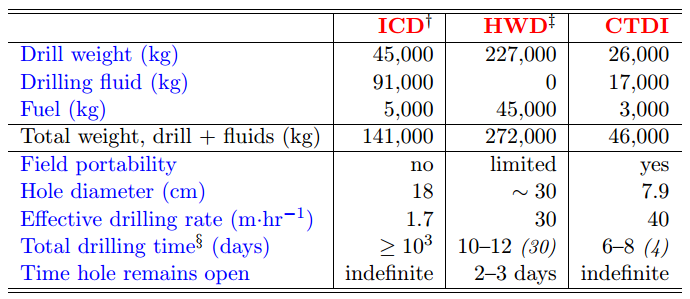
\includegraphics[width=0.7\textwidth]{figures/mlh/table_ice_core_drilling}
  \caption{Comparison of the weights and times required to drill a 3.5-km borehole through ice using ice-coring, hot-water, and CTDI drilling systems.}
  \label{tab:ice_core_drilling}
\end{figure}

Figures \ref{fig:ICD}, \ref{fig:HWD} and \ref{fig:CTDI} illustrates the three methods presented in table \ref{tab:ice_core_drilling}.

\begin{figure}[htb]
  \centering
  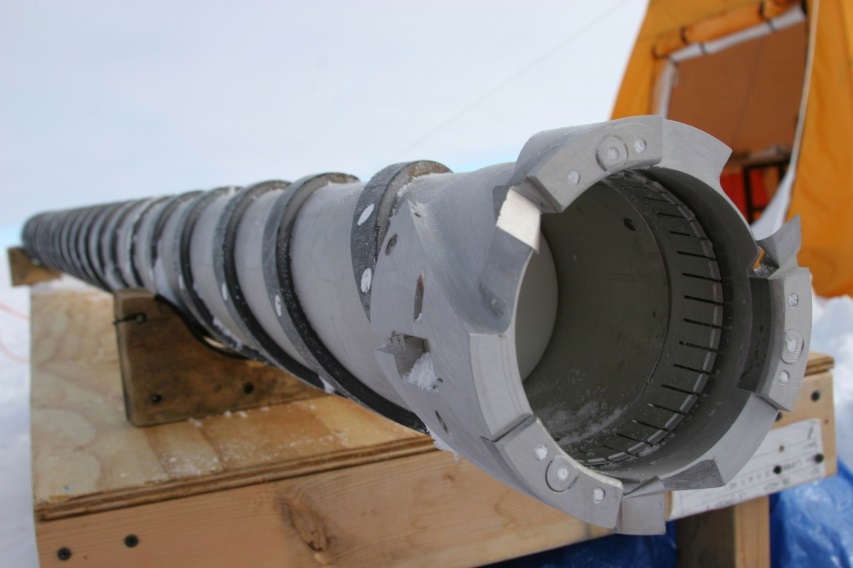
\includegraphics[width=0.5\textwidth]{figures/mlh/ICD}
  \caption{The hollow drill of an Ice Core Drilling, which enables researchers to retrieve pure ice core samples.}
  \label{fig:ICD}
\end{figure}
\begin{figure}[htb]
  \centering
  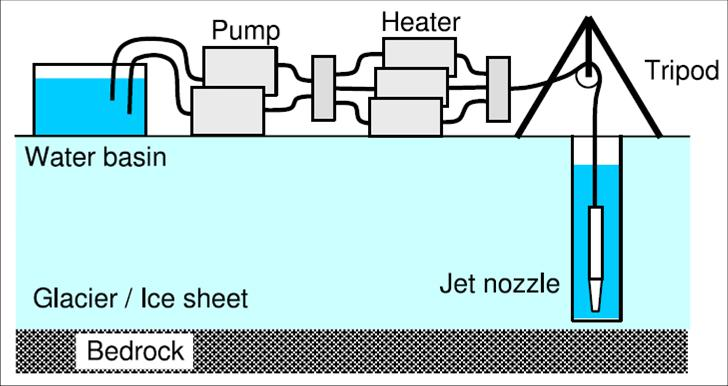
\includegraphics[width=0.5\textwidth]{figures/mlh/HWD}
  \caption{Principles of Hot Water Drilling in ice.}
  \label{fig:HWD}
\end{figure}
\begin{figure}[htb]
  \centering
  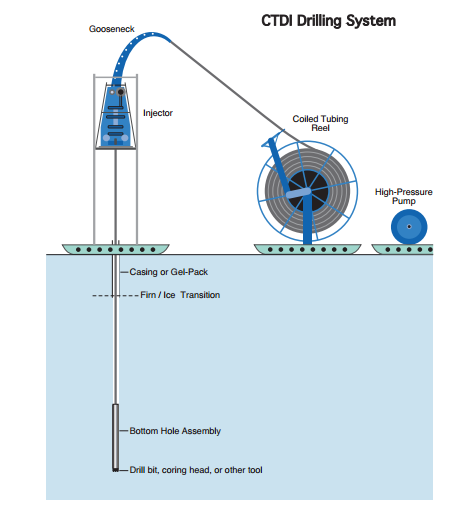
\includegraphics[width=0.6\textwidth]{figures/mlh/CTDI}
  \caption{Principles of Coiled Tube Drilling in Ice.}
  \label{fig:CTDI}
\end{figure}

\subsection{Chemical Drilling}

\subsection{Explosive Drilling}

\autsubsection{Sputtering Drilling}{Paul Connetable}

\subsubsection{Sputtering physics and research on sputtering on water ice}

The concept of sputtering is to send particles with a high kinetic energy on a solid, in order to eject the surface particles of the solid. Generally, the particles sent on the solid are ions, but it can be any atom. It is the energy exchange between the incoming particle and the surface molecules which eject these particles. In order to be ejected, the energy brought to the solid surface must exceed the binding energy of its molecules. A single particle sent can eject several atoms or particles at once, and is called the sputter yield. The sputter yield depends on the ion incident angle, its mass, its velocity, and the mass and the binding energy of the solid atoms. Some research about sputtering on water ice has been made in \cite{baragiola2003sputtering}.
In this research, the sputtering yield of water ice has been measured under several conditions, and for several types of ions, and several very interesting results have been obtained:

\begin{itemize}
    \item{The sputtering yield of water ice is constant below 100K for $O_{+}$, $AR_{+}$ and $HE_{+}$ ions, as shown in Figure \ref{sputtering30kev};}
    
    \item{The sputtering yield of water ice is dependent on the fluence, (i.e. the concentration of ions sent on the ice surface per surface unit) for $O_{+}$ ions only, among the different ions tested. It increases from 11 to 14 molecules as shown in Figure \ref{sputteringfluence}}

    \item{The influence of the incoming ion's energy on the sputtering yield is shown in Figure \ref{sputteringenergy} below. One can observe that thresholds appear for $O_{+}$ and $H_{+}$ ions in the displayed energy interval.}
\end{itemize}
    
\begin{figure}[htb]
\centering
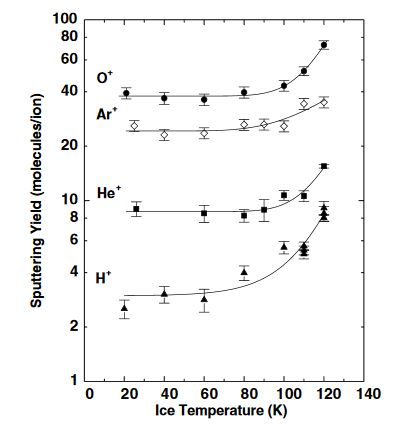
\includegraphics[width=8cm, height=10cm, clip]{Paul/sputtering30kev.JPG}
\caption{Influence of ice temperature on the sputtering yield}
\label{sputtering30kev}
\end{figure}
    
\begin{figure}[htb]
\centering
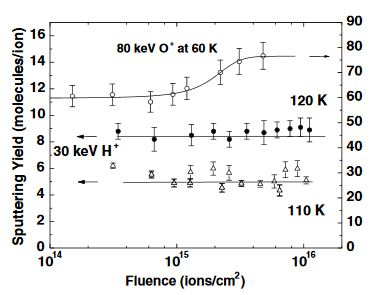
\includegraphics[width=10cm, height=8cm, clip]{Paul/sputteringfluence.JPG}
\caption{Influence of fluence on the sputtering yield}
\label{sputteringfluence}
\end{figure}
    
\begin{figure}[htb]
\centering
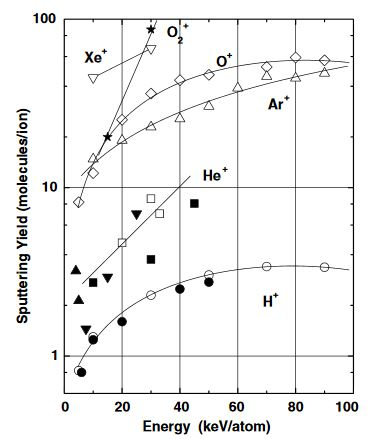
\includegraphics[width=8cm, height=10cm, clip]{Paul/sputteringenergy.JPG}
\caption{Influence of the incoming ion energy on the sputtering yield}
\label{sputteringenergy}
\end{figure}


\subsubsection{Conclusion on the metod}

These results allow a quick calculation on the energy needed to drill through a certain depth of ice. To erode 1 liter of ice at 60K, the total energy needed by sputtering is of approximately $10^{7}~kJ$. As a comparison, the energy needed to evaporate one liter of ice is of around $3~\times10^{3}~kJ$. It is to be expected that the total energy required to just melt and evaporate ice is way smaller than the energy needed to erode it by sending ions on it, but these results still show an enormous difference in the energy needed. This very rough simulation has been done while assuming the use of $O_{+}$ ions, and assuming a sputtering yield of 20 atoms per ion. Such a sputtering yield is achievable for around ions at 20 keV according to Figure \ref{sputteringenergy}.

Sputtering drilling has other drawbacks for our mission:
\begin{itemize}
\item{this technique would create a contamination of the middle~;}
\item{using this technique would mean to bring a material reserve, which would be used to sputter the ice. This reserve would weight a lot.}
\end{itemize}

Actually, sputtering has only been researched on very thin layers of ice. In \cite{baragiola2003sputtering}, the maximum thickness of ice tested was of 250 nm.This method is not the best to drill holes, but is rather commonly used to erode surfaces and deposit thin layers of material on manufactured products. this is why this method is not the one chosen on our mission on Europa.

\autsubsection{Laser Drilling}{Bhaaeddin Alhomsi and Paul Connetable}

Lasers may provide another methodto dig through the layer of ice. High-power lasers exceeding 10 kW have been developed and widely used for industry (Gapontsev et al., 2009; Richardson et al., 2010; Fujita et al., 2010). For example, a recent laboratory test using a 1.6-kW pulsed Nd:YAG 1.064 $\mu$m wavelength laser beam determined the energy required to spall, melt, and
vaporize several rock samples for oil and gas well drilling. The required energy (specific energy) depends on the absorption properties of each rock sample as well as the reflective properties of the rock surface  (Gahan and Parker, 2001; Xu et al., 2003). A new laser-mechanical bit for laser spallation of rock to give an optimum drilling mechanism
was found to reduce rig time and increase drilling efficiency (Pooniwala, 2006).More recently, a 20-kWlaserwas delivered through a 1500 m-long optical fiber cable and shown to be able to efficiently drill oil and gas wells (Hecht, 2012). Finally, in the project VALKYRIE,
ice was drilled by a self-contained "intelligent ice penetrator", a 5 kW laser at 1070 nm wavelength (Siegel et al., 2013)(Stone et al., 2014).
Test of VALKYRIE between 2010 and 2013 used high-power optical energy transfer over km-scale distances and tested the feasibility of a vehicle deployed optical waveguide. Thus, a laser-drill system may be useful for ice-sheet applications, including the search for life in extreme environmental conditions here on Earth as well as outer planets.
With continual improvements, laser drilling may develop advantages over other methods for ice.We investigate here the behaviour of laser melting of ice and snow with an infrared laser for the potential use as a drill.

\subsubsection{Characteristics of light absorbance in ice}

The first step before selecting a laser is to analyze the spectral absorption of the medium we want to dig through. Therefore, the ice transmittance spectrum is displayed in Figure \ref{IceAbsorbance}. One can observe on this figure peaks of absorption, at around $10^{-5}~m$, and around $6\times10^{-5}~m$. The best suited lasers for digging through ice would have to emit at these frequencies.

Hence, we use a $CO_2$ laser, which is a relatively inexpensive common infrared gas laser (Patel, 1964) with fundamental lines from 9.2 to 10.8 $\mu$m and used in both pulse and continuous wave (CW) mode. For ice, an earlier study demonstrated the potential of $CO_2$ laser irradiation to help breakup nautical sea-ice (Clark et al.,  1973), but the laser has apparently not previously been used for snow and ice drilling.

\begin{figure}[htb]
\centering
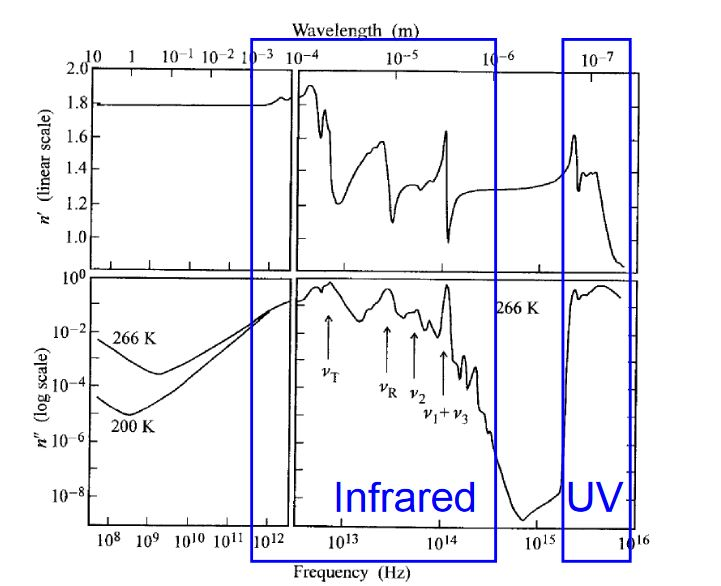
\includegraphics[width=.48\textwidth]{figures/laser-drilling/iceabsorbance}
\caption{Reported values of transmittance in ice}
\label{IceAbsorbance}
\end{figure}

The absorption of light in ice depends on the complex refractive index of ice. According to data in a previous study (Warren and Brandt, 2008), the absorption coefficient of ice significantly increases from the near- to mid-infra-red region, reaching a value of about $\unit[628.3]{cm^{-1}}$ at the $CO_2$ laser wavelength of 10.6 $\mu$m. Ice absorbs almost 100\% of the light intensity at 10.6 and 1.064 $\mu$m within a penetration distance of 0.01 and 2 cm, as shown in Figure \ref{fig:bh1}.

\begin{figure}[htb]
\centering
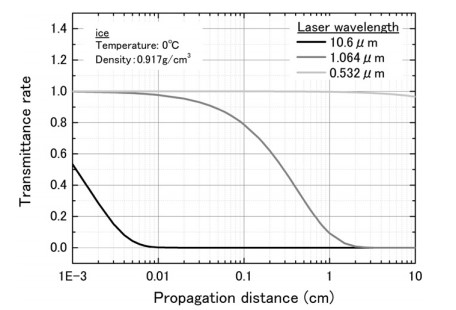
\includegraphics[width=.48\textwidth]{figures/laser-drilling/bh1.jpg}
\caption{Characteristics of light absorbance in ice}
\label{fig:bh1}
\end{figure}

\subsubsection{Melting studies of ice and snow by $CO_2$ laser}

A $CO_2$ laser can be used to melt ice. The $CO_2$ laser at 10.6 $\mu$m (25.5 W) and a beam diameter of 1.0 cm, a wavelength at which ice strongly absorbs, to drill (via melting) through ice. The resulting drilling speed is measured at several irradiation intensities, ice-snow densities, and beam angles relative to the horizontal axis.
The melting speed increases with increasing laser intensity and with decreasing ice density, as shown in Figure \ref{fig:bh2}. The melting speed ratio between ice ($\unitfrac[917]{kg}{m^3}$) and the lowest-density snow ($\unitfrac[153]{kg}{m^3}$) is 4-5, slightly less than the value of \~6 expected from the density ratio \cite{lasermelt}. The reason for this discrepancy could be explained by the snow having a greater reflectivity than solid ice. The melting speed decreases with increasing snow density.

\begin{figure}[htb]
\centering
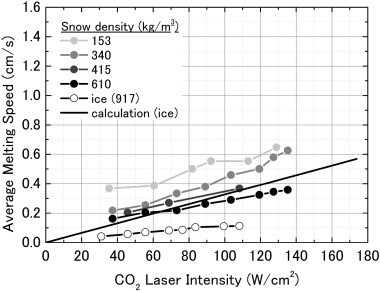
\includegraphics[width=.48\textwidth]{figures/laser-drilling/bh2.jpg}
\caption{Relation between laser intensity and melting speed}
\label{fig:bh2}
\end{figure}

\subsubsection{Results}

Unfortunately, the experimental results indicate that the melt-water accumulates in the hole and reduces the melting speed of ice and a pump system could not be installed due to a high distance.
Moreover, since the energy source brought in the penetrator is a RTG, using a laser would require to transform the thermal energy produced by the RTG in electric energy. Such a conversion has an efficiency of about 20~\%. If we add to that the fact that the best $CO_{2}$ lasers also have efficiencies up to only 20~\%, the best efficiency achievable on this drilling method is of about 4~\%with the current technology. This is still while assuming that the ice absorbs all of the energy sent by the laser, which is not the case. It means that the efficiency of such a drilling method would be extremely low, and thus not indicated for our mission.
In future studies, it will be necessary to investigate quantitatively several additional factors. These include the optical-fiber coupled laser intensities required for deep drilling, and a method to pump melted water. Despite these hurdles, laser drilling is a promising technology for ice drilling. Lasers are indeed capable of delivering very high powers precisely. Furthermore, the main reason for low $CO_{2}$ lasers' efficiency is the power consumed for cooling the body of the laser. This efficiency could then go up if a laser specifically designed for our mission was done, since it could use the cold surroundings of the penetrator to cool down.


\subsection{Light Concentration Drilling}

\subsection{Melting}

* Water transportation from tip to the end of the penetrator (ref section about convection flow)

* Should measure flow of the water - descent rate

* Water flow to the instruments. Will have to use a pump in order to increase the flow rate.

* Measure conductivity of the water.

%\subsection{Melting Considerations} % Lukas, KSL
\autsubsection{Thermal Drilling}{Lukas Christensen}\label{sec:temp_simulation}
Most drilling methods convert electrical energy to some other form like, for example, kinetic or electromagnetic energy. During this conversion some amount of energy will be lost as heat to the environment and therefore not contribute to the drilling process. With thermal drills, however, this is not an issue since it is the heat itself that is used for the penetration process. This means that thermal drills are highly efficient, even though more energy is needed to melt a given material than to, say, break up its structure mechanically. Additionally, they are very simple to design and implement, since all that is needed is basically a heating element and an enclosure. It is even possible to use radioisotope thermal generators for the heating source, eliminating the need for any energy conversion in the drilling process.\\

\noindent
The calculations presented in section \ref{sec:IceTemperatureProfile} provide an initial estimate of the amount of thermal energy that is needed to penetrate the Europan ice sheet. Based on this, it would seem that melting through the ice can be achieved within realistic mission durations, however, more detailed calculations that take thermal loss in to account are needed before it is possible to conclusively choose a drilling method and optimize the design of the mission. \\

\noindent
A simulation has therefore been developed to accommodate this issue, however, it should be noted that a number of assumptions have been made in order to simplify the calculations somewhat. These include:
\begin{itemize}
	\item The ice sheet is homogeneous.
	\item The pressure variation throughout the ice has a negligible impact on the thermal characteristics.
	\item The bore hole closes and causes pressure build up to Earth atmospheric levels sufficiently fast that sublimation can be disregarded.
	\item The ice consists of pure water with no contents of salt or other pollutants.
\end{itemize}
The first assumption is probably not very realistic, but cracks in the ice and similar inhomogeneities will disrupt the conductive flow of heat thus result in a lower amount of heat transfer compared to the simulation results. This means that while the result of the simulation might not be completely realistic, it will represent a worst case scenario since less energy will likely be lost to the ice in reality. \\

\noindent
The second assumption should not result in significant deviations from reality as the melting point of water as well as the latent heat of fusion does not change significantly in the range of 1 to 100 atmospheres, which is the expected pressure range bearing in mind the third assumption. On the phase diagram presented in Figure \ref{fig:waterPhase} this is shown quite clearly with the boundary line between the solid and liquid state being near vertical at 273 K in the range of 1 kPa to 10 MPa.\\

\begin{figure}[ht]
	\centering
	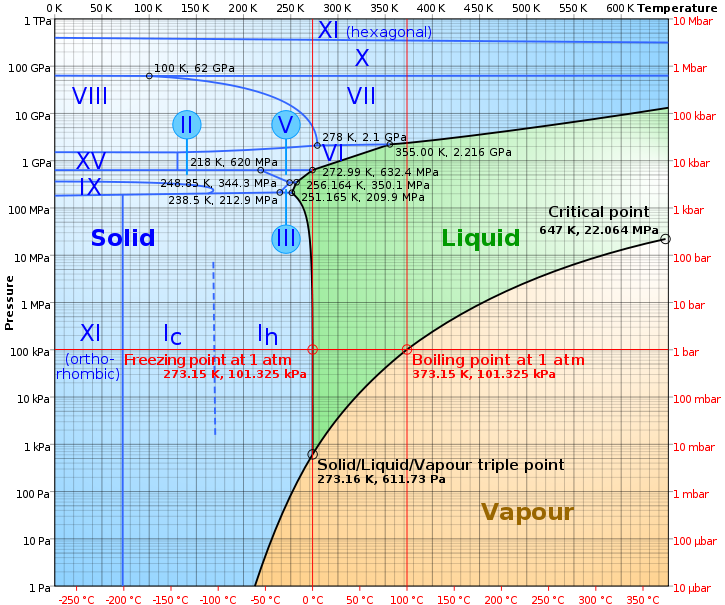
\includegraphics[width=8cm]{figures/LAMC/waterPhase}
	\caption{Phase diagram of water. Source: \url{http://math.ucr.edu/home/baez/chemical/725px-Phase_diagram_of_water.svg.png}}
	\label{fig:waterPhase}
\end{figure}

\noindent
The third assumption is probably fairly realistic considering that a relatively narrow penetrator ($\approx$ 20 cm diameter) is being considered. Naturally, at the beginning of the drilling process the ice will have to undergo sublimation as the pressure is very close to vacuum, however, the sublimated ice particles will most likely adhere to the inner surface of the bore hole and make it narrower and narrower. After a while the bore hole will then close completely and pressure will start to build until sublimation is replaced by melting. How quickly this happens it quite critical considering that the sublimation energy of ice is about 7 times\cite{website:engineeringToolbox} that of the melting energy. Experiments are needed to determine how exactly this progresses, but for now the simulation should still provide a decent estimate of the penetration time.\\

\noindent
The fourth assumption is most certainly not realistic and it will in all likelihood have a great deal of impact on the result, however, the implications of it will be discussed further in a separate section.

\subsubsection{Theory}
In order to evaluate the temperature evolution of a continuous fluid a good starting point is the equation of conservation of energy. For an incompressible fluid with no internal forces this is given by
\begin{equation}
\rho C \left( \mathbf{v} \cdot \nabla T + \frac{\partial T}{\partial t} \right) = \nabla (K \nabla T) + q 
\end{equation} 
Where $\rho$ is the density, $C$ is the heat capacity, $\mathbf{v}$ is the velocity of the fluid, $T$ is the temperature, $K$ is the thermal conductivity, and $q$ is added heat\cite{article:barr2014a}. Assuming no internal motion and a near constant thermal conductivity this reduces to
\begin{equation}
\label{eq:thermal1}
\frac{\partial T}{\partial t} = \frac{1}{\rho C}\left( K \nabla^2 T + q \right)
\end{equation}
For the case of a penetrator melting through the ice this equation becomes exceedingly difficult to solve analytically as the ice changes state during the melting and the heat source moves as a function of this. For this reason, it is advantageous to discretize the equation in order to facility computer simulations, which results in\\
\begin{equation} \label{eq:thermal2}
T_{k+1} \approx T_{k} + \frac{\partial T_{k}}{\partial t}\Delta t = T_{k} + \frac{\Delta t}{\rho_k C_k}\left( K_k \nabla^2 T_{k} + q_{k} \right)
\end{equation}
With $\Delta t$ being a small time step and $k$ being the current iteration number. Note that all the quantities in this equation, except $\Delta t$, need not be constant all over, but can vary spatially. Of course, ideally $K_k$ should only exhibit small variations in order to satisfy the earlier approximation. This is not strictly true at the interface between ice and water as there will be a discontinuous jump from $\SI{0.57}{\frac{W}{m K}}$ in the water to $\SI{2.22}{\frac{W}{m K}}$\cite{website:engineeringToolbox} in the ice, but the approximation should still be able to provide decent results.\\

\noindent
Once a volume $V$ of ice reaches its melting temperature, the amount of heat that is needed to convert it into water is equal to
\begin{equation}
Q_{melt} = \rho V L_{fus}
\end{equation}
Where $L_{fus} = \SI{333.5}{\frac{kJ}{kg}}$ is the latent heat of fusion of water\cite{article:biele2011a}.

\subsubsection{Implementation}
The actual simulation program have been implemented using Matlab as it easily accommodates scientific calculations on large matrices. The actual simulation algorithm is run on a 51x60x60 temperature matrix with each voxel representing a volume of 0.5x0.1x0.1 $\SI{}{m^3}$, totaling in a 25.5x6x6 $\SI{}{m^3}$ section of the ice sheet. As the heater melts through the ice, the grid moves with it thus eliminating the need for simulating the entire ice sheet at all times. The processing performed on the volume section is outlined in Figure \ref{fig:iceSimFlow}.\\

 \begin{figure}[ht]
 	\centering
 	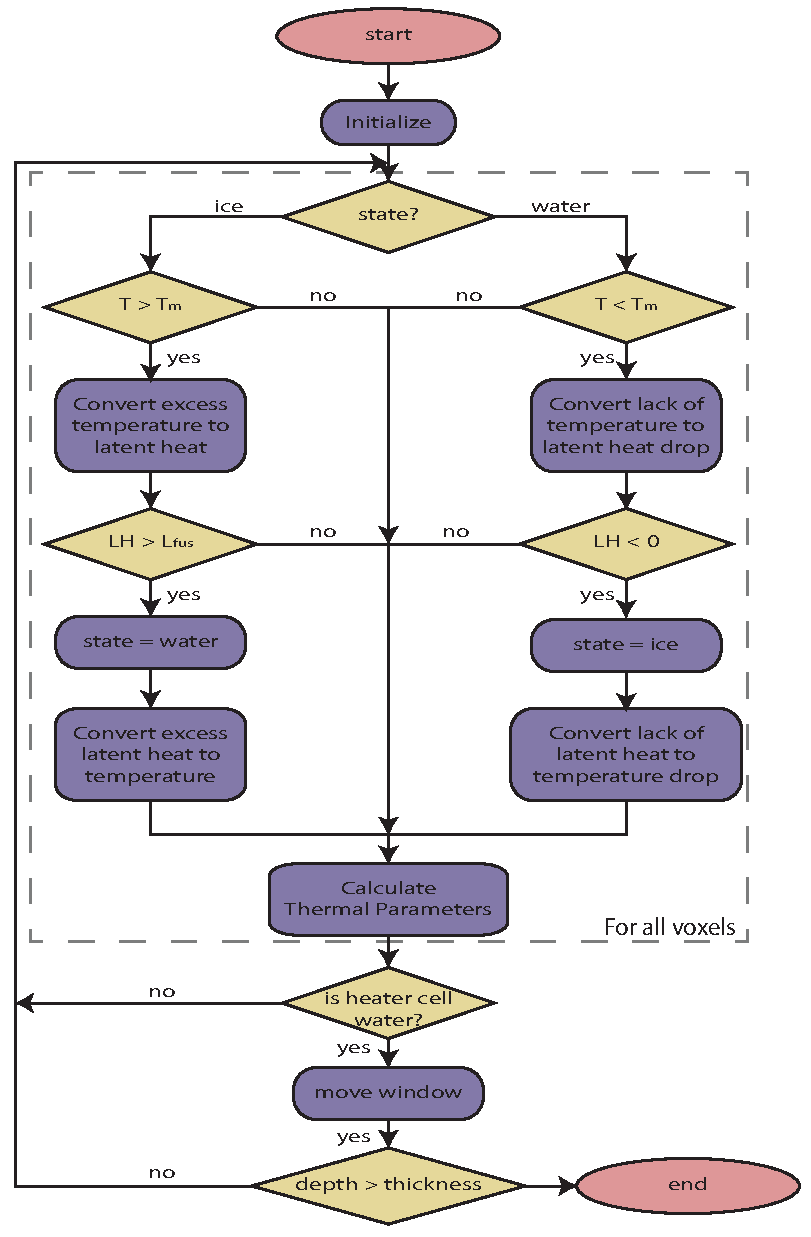
\includegraphics[width=.55\textwidth]{figures/LAMC/iceSimFlowchart.pdf}
 	\caption{Flowchart of the ice melting simulation.}
 	\label{fig:iceSimFlow}
 \end{figure}
 
\noindent
First, the change in temperature is calculated according to equation \ref{eq:thermal2} with the Laplacian being calculated using the Matlab command \texttt{del2()}. It is noteworthy that \texttt{del2()} actually, for whatever reason, returns $\frac{\nabla^2}{6}$ when working with 3D-coordinates. This change is then added to the current temperature value.\\

\noindent
At this point, the simulation branches out depending on whether a given grid cell is made up of water or ice. If it is an ice voxel, a check is made to see if the current temperature is above the melting point of ice. If this is the case, the excess temperature is converted to latent heat and stored in a separate matrix. If the latent heat is now above $L_{fus}$, the voxel state is set to water and the excess heat is converted to a temperature change and added to the current voxel.\\

\noindent
For a water voxel, the temperature is checked to see if it is below the melting point of water. If true, the temperature deficiency is converted and subtracted from the latent heat. If the latent heat now drops below 0, the cell is converted to ice and the negative latent heat is subtracted from the temperature (after being converted, of course).\\

\noindent
With the temperature and the state of each voxels being determined, the thermal parameters of each cell is determined by interpolating between points in a dataset that includes heat capacity, thermal conductivity and density for water and ice for a range of different temperatures. The dataset has been put together by combining information acquired from \cite{website:engineeringToolbox}. It should be noted that this data only covers the temperature interval 183-366 K and linear extrapolation has been used for temperatures outside of this range.\\

\begin{figure}[ht]
	\centering
	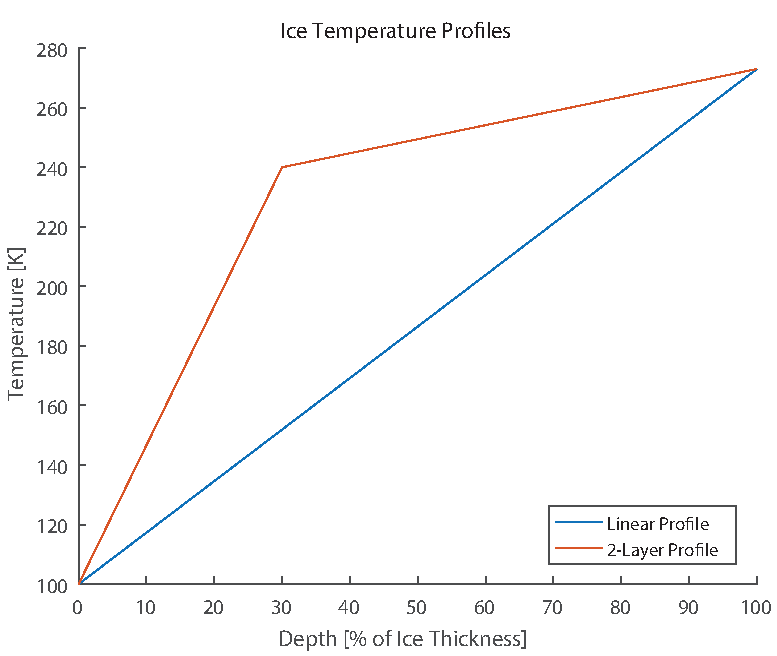
\includegraphics[width=.5\textwidth]{figures/LAMC/iceTempProfiles.pdf}
	\caption{The two temperature profiles used in the simulation: the linear based on calculations, and an approximated 2-layer profile based on the literature.}
	\label{fig:iceTempProfiles}
\end{figure}

\noindent
This basic flow is run for every voxel at every time step, until the heater makes it way through the ice sheet. The actual heater is implemented by injecting power in to a number of voxels that represent the extends of the heater. In the present configuration these consists of 4 cells located next to each other (2 by 2), however, not all the power is added to these. In order to accommodate the fact that the heating is distributed along the length of the penetrator, some of the power is injected in to the cells immediately above the heater. The exact amount is determined by a coupling coefficient, which is set to 99 \% in the used configuration meaning that 99 \% of the power is added to the heater cells and 1 \% percent is added to cells above. \\

\noindent
The amount of energy lost to heating the ice matrix and therefore not directly used to melt the ice below the penetrator is heavily influenced by this coupling coefficient. The used value was chosen as it seemed to match well with calculations that will be detailed in the validation section. To achieve a completely realistic result, real world experiments are needed to determine what the coupling coefficient should be set to.\\

\noindent
As soon as the heater voxels are converted to water, the entire simulation window together with the heater position is moved down by one increment of the vertical resolution. At the same time a depth variable is incremented by the same amount. Once this reaches the preset thickness of the ice sheet, the simulation is stopped. \\

 \begin{figure}[ht]
 	\centering
 	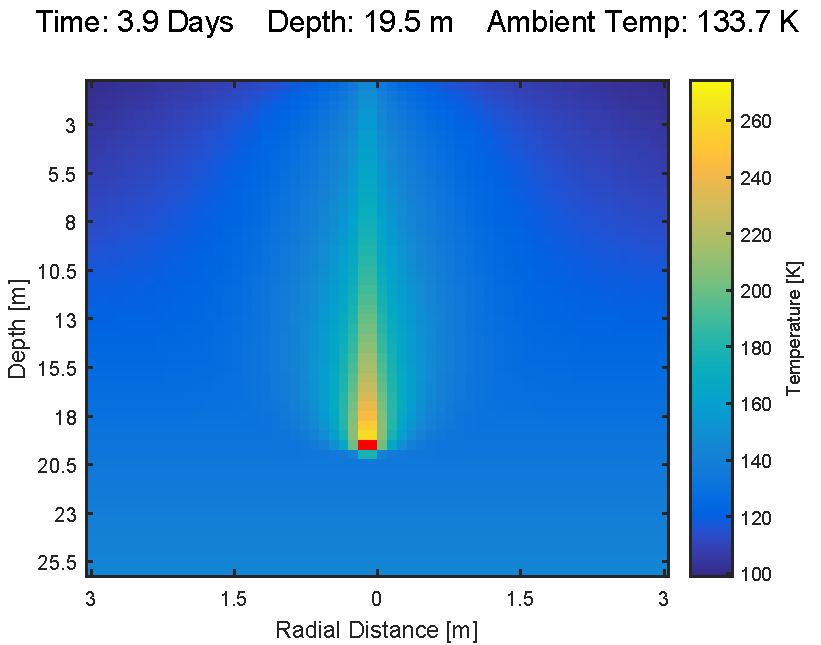
\includegraphics[width=0.5\textwidth]{figures/LAMC/snapshot.pdf}
 	\caption{Snapshot from the simulation program. This example is running with an ice thickness of 100 m, a linear temperature profile and a heater power of 2000 W. The red pixels indicate where the ice has melted and turned in to water. Videos of the running simulation are available at \url{https://www.youtube.com/watch?v=Rr-ucW9Br4A} and \url{https://www.youtube.com/watch?v=b72MfGw1ZE8}}
 	\label{fig:simSnapshot}
 \end{figure}

\noindent
The temperature that is loaded into the grid when the simulation is first initialized, as well as the temperature that is used to update the grid every time it moves, is calculated using a chosen temperature profile. Currently two different profiles have been implemented namely the ones presented in sections \ref{sec:IceTemperatureProfile} and \ref{sec:IceTemperatureProfile2}: the linear one based on calculations, and an approximation of the two layer model with a thin cold layer followed by a thick warm layer. These profiles are plotted in Figure \ref{fig:iceTempProfiles}.\\

\noindent 
A snapshot created during a run of the simulation is displayed in Figure \ref{fig:simSnapshot}, clearly showing how a large part of the heating energy is being used to heat up the surrounding ice. The source code for the simulation is included in appendix \ref{app:iceSimCode}.


\subsubsection{Results}
Running the simulation with a constant heating power for a number of different ice thicknesses, it is clear that the penetration time is directly proportional to the ice thickness. This means that the simulation can be run with a thickness of just 100 m to reduce run times and still provide results that can be extrapolated to any arbitrary thickness. Furthermore, it is the power to cross-sectional area ratio that the determines the penetration time, meaning that only a few heating voxels are needed to get seemingly accurate results that can represent any given penetrator size. Running the simulation for a number of different heating values, but with a fixed heater size, results in Figure \ref{fig:simResults}.

\begin{figure}[ht]
	\centering
	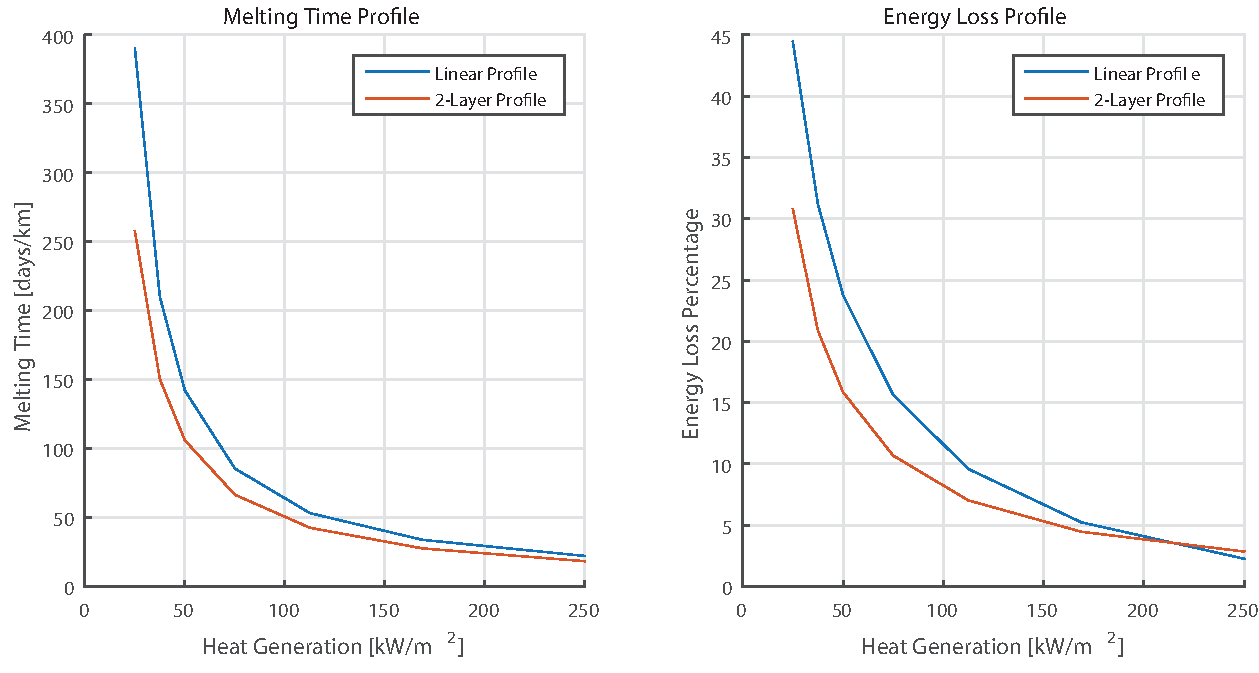
\includegraphics[width=.9\textwidth]{figures/LAMC/simResult.pdf}
	\caption{Result of the melting simulation. The left plot shows the penetration time per kilometer of ice for the two temperature profiles with varying heating densities, while the right shows the associated losses.}
	\label{fig:simResults}
\end{figure}

\noindent
The x-axis on the two graphs is equal to the total heater power divided by the cross-sectional area of the penetrator and loss percentage has been calculated as the ratio between the used energy and the energy needed to melt only the ice column the penetrator travels through. \\

\noindent
It can be seen that the both penetration time and loss percentage follows something similar to an exponentially decreasing curve. This means that the higher the power density the better, however, a point of diminishing returns is reached at around a heating density of $\SI{85}{\frac{kW}{m^2}}$. \\

\noindent
The working model of the penetrator has a 2 kW heater and a diameter of 20 cm meaning a heating density of $\SI{64}{\frac{kW}{m^2}}$ resulting in a loss of 19 \% and a penetration time of $\SI{111}{\frac{days}{km}}$ for the linear temperature profile, and 13 \% and $\SI{84}{\frac{days}{km}}$ for the 2-layer profile. So, for these penetrator dimensions it should be possible to design a mission with a realistic lifetime that can reach the bottom of the ice sheet. Granted, this requires that the ice has a modest thickness; with much more than 5 km of ice multiple years are needed for the penetration which is probably not realistic.\\

\noindent
If the ice sheet is found to be unreasonably thick, one option will be to reduce the diameter of the penetrator. Changing the design to a diameter of 15 cm instead results in penetration times of $\SI{42}{\frac{days}{km}}$ to $\SI{53}{\frac{days}{km}}$, depending on the temperature profile. This would enable a doubling of the ice thickness while maintaining the same mission duration. Of course, this would require a redesign of the mission, but the option is available. Alternatively, increasing the heater power by 80 \% would result in the same gain in power density. 

\subsubsection{Verification}
The simulation has provided results that show the mission to be possible, however, these results need to be verified to make sure that the simulation reflects the real world.\\

\noindent
According to Biele et al. (2011)\cite{article:biele2011a}, the amount of power that is lost to heating up the ice around a heating element is equal to
\begin{equation}
P_{cond}=\frac{4 K (T_m-T) }{R\pi^2}(2\pi R)\times \int_{0}^{H}\int_{0}^{\infty}\frac{
e^{-\kappa u^2 s/v}
}{
u\left[J_0^2(R u) + Y_0^2(R u)\right]
}duds
\end{equation}
Where $T_m$ is the melting temperature, $T$ is the temperature of the ice, $R$ is the radius of the heater, $H$ is the length of the heater, $\kappa=\frac{K}{\rho C}$ is the heat diffusion coefficient, $v$ is the downward speed of the heater, and $J_0^2$ and $Y_0^2$ are the first two Bessel functions of zero'th order. The total power needed to move at a given speed is then equal to
\begin{equation}
P_{tot} = A\rho v(C(T_m-T) + L_{fus}) + P_{cond}
\end{equation} 
With $A=\pi R^2$ being the cross-sectional area of the heater. In the case of the penetrator, the velocity is not known, but the total power is. By numerically solving $P_{tot}$ equal to some given power, the velocity, and by extension $P_{cond}$ can be determined. Afterwards, the velocity can be integrated to find the penetration time, and the total loss can be calculated from $P_{cond}$. Performing this process for a number of different heater powers and the two temperature profiles results in Figure \ref{fig:verificationResult}.

\begin{figure}[ht]
	\centering
	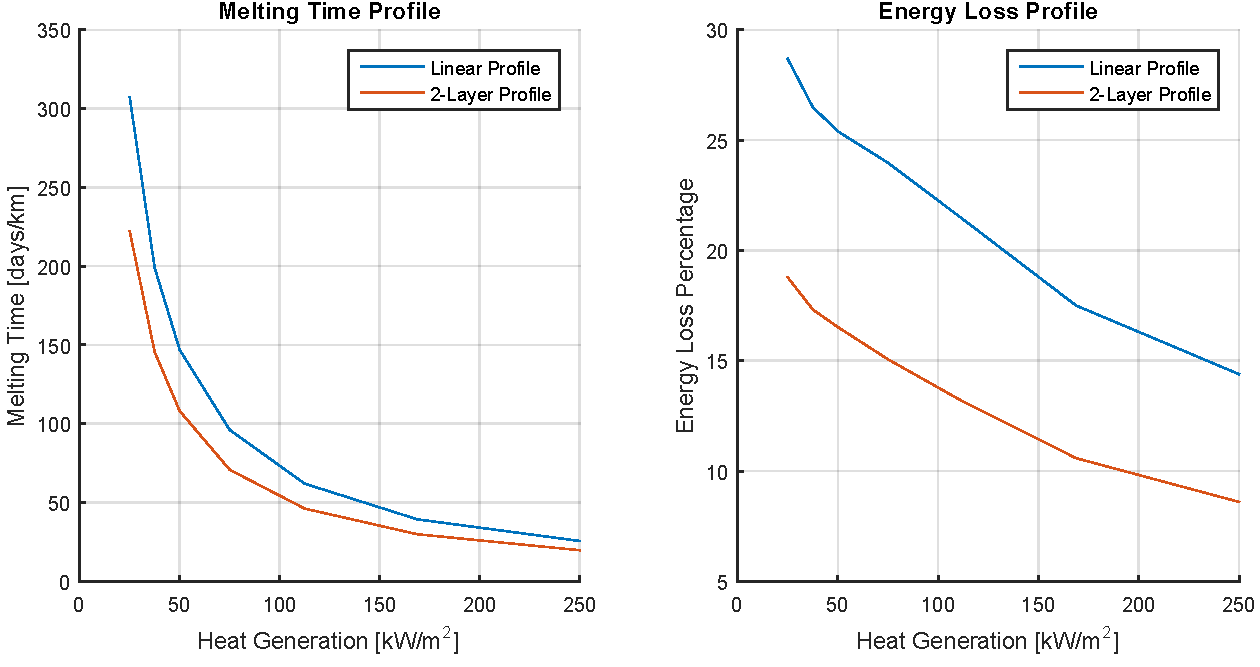
\includegraphics[width=.9\textwidth]{figures/LAMC/verificationResult.pdf}
	\caption{Result of solving the loss power equation for different heater densities. The left plot shows the penetration time per kilometer of ice. The right shows the calculated losses. Cross-section of $\SI{0.04}{m^2}$ was used together with a heater length of 0.15 m.}
	\label{fig:verificationResult}
\end{figure}

\noindent
By comparing this to Figure \ref{fig:simResults}, it is clear that there are discrepancies between the simulated and the calculated losses: For low power densities the simulation overestimates the losses, and for the high densities the simulation results in much too low losses. Even so, there is a very good match in the penetration times, with a deviation below $\SI{8}{\frac{days}{km}}$ for most power densities and with an absolute maximum at the lowest heating density of  $\SI{80}{\frac{days}{km}}$. This indicates that the simulation does, indeed, provide realistic results. The reason that the penetration times can be similar, even though the losses are different, is probably that the difference in loss is largest at the high power densities where the penetration time is the shortest. This means that the errors have less time to accumulate resulting in lower overall differences.\\

\noindent
To generate these graphs a cross-sectional area of $\SI{0.04}{m^2}$ and a heater length of 0.15 m was used. The choice of the heater length is meant to reflect that most of the heating power will be situated in the front of the penetrator. Of course, this is not an entirely physically correct picture, since some power will distributed through the penetrator to keep the instruments at a pleasant temperature and to make sure that the top of the does not get stuck in refreezing ice. Additionally, the density, heat capacity and thermal conductivity are assumed to be constant throughout the ice, further simplifying the picture. However, seeing as the calculations and the simulations provide very similar results it is probably safe to assume that the results can be trusted to reflect the real world, at the very least as a first approximation.\\

\subsubsection{Salinity} \label{sec:iceSalinity}
As previously mentioned, the ice will certainly include some amount of salts and other pollutants, however the actual concentration and composition is still unknown. These pollutants will most definitely have an effect on the penetration time, but it is difficult to find numerical values for the thermal properties at different salinities and temperatures - especially for other salts than sodium chloride. However, \citet{book:thomas2009sea} states that for sea ice these parameters can be approximated by empirical formulae:\\

\noindent
For the thermal conductivity, the following relation holds
\begin{equation}
K_{si}=\frac{\rho_{si}}{\rho_i}\left(2.11 - 0.011 T + 0.09 \frac{T}{S} - \frac{\rho_{si}-\rho_i}{1000}\right)\SI{}{\frac{W}{m K}}
\end{equation}
Where $\rho_{si}$ is the density of sea ice (on average $\SI{910}{\frac{kg}{m^3}}$\cite{article:timco19961}), $\rho_i$ is the density of pure water ice ($\SI{927}{\frac{kg}{m^3}}$), $T$ is the temperature measured in $^\circ C$ and $S$ is the salinity in ppt.\\
Similarly, the heat capacity can be approximated as
\begin{equation}
C_{si} = \left(2.11 + 17.2 \frac{S}{T^2}\right)\SI{}{\frac{kJ}{kg K}}
\end{equation}
And finally, the latent heat of fusion is given by
\begin{equation}
L_{si}=\left(333.4-2.11T-0.114S+18.1\frac{S}{T}\right)\SI{}{\frac{kJ}{kg}}
\end{equation}

\noindent
Plotting these equations for varying temperatures and salinities results in Figure \ref{fig:iceSalinity}.
\begin{figure}[ht]
	\centering
	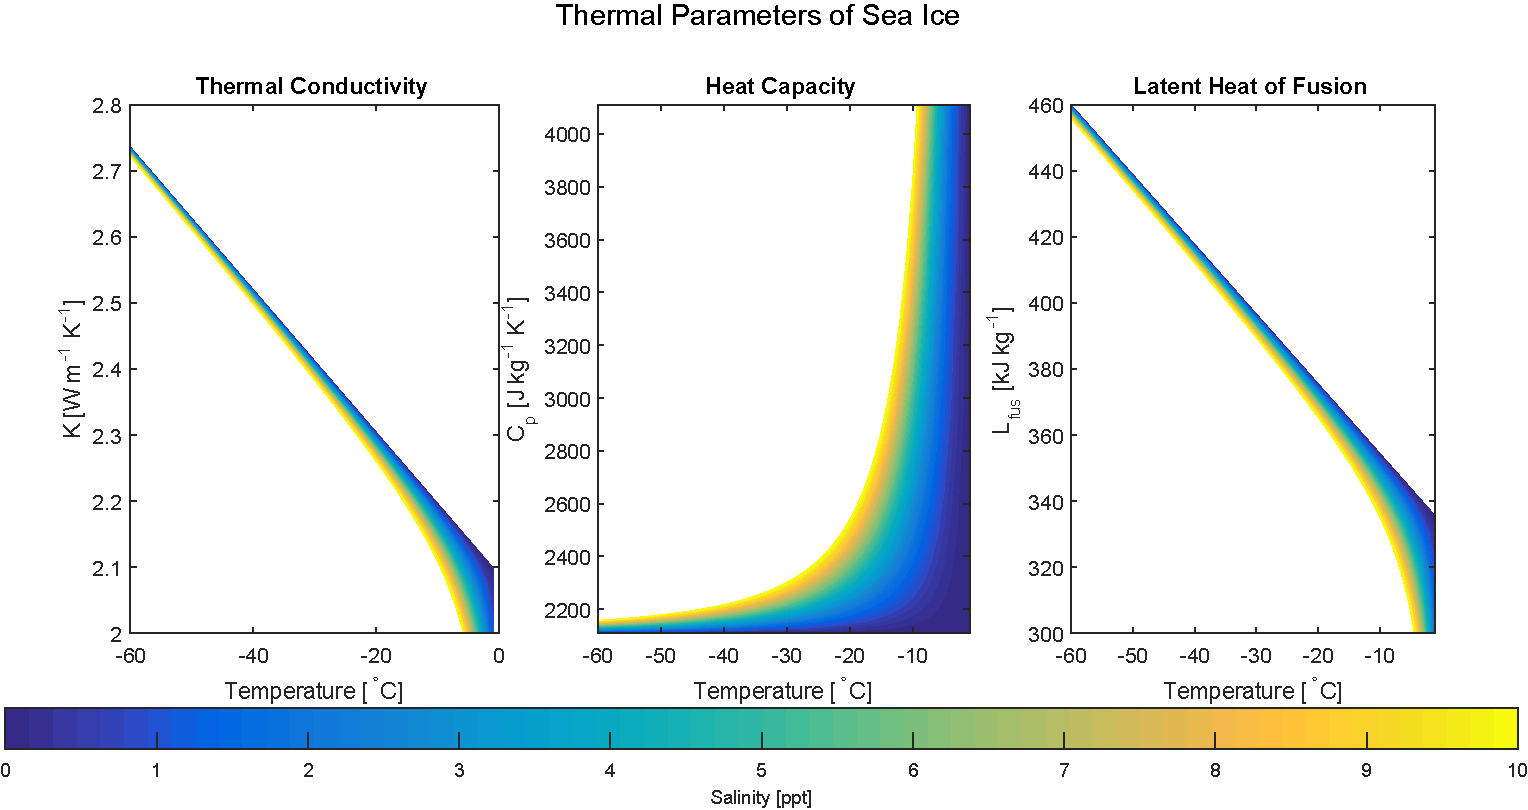
\includegraphics[width=.9\textwidth]{figures/LAMC/salinity}
	\caption{Thermal parameters of sea ice as a function of temperature and salinity.}
	\label{fig:iceSalinity}
\end{figure}
As can be seen, both the thermal conductivity and the latent heat of fusion decreases with increasing salinity, while the heat capacity increases. \\

\noindent
The increase of the heat capacity will result in more energy being needed to heat up the ice, which will work towards increasing the penetration time. On the other hand, the decreasing heat of fusion and thermal conductivity will mean that less energy is needed for the melting process and there will be an overall lower loss as less heat is conducted away from the penetrator.\\

\noindent
Seeing as the latent heat accounts for some 65-80\% of the ideal amount of energy needed to melt through the ice, it would seem that the decrease in the latent heat of fusion alone would outweigh the increase in heat capacity. Combining this with the decrease in thermal conductivity as well strongly indicates that salinity will actually work in favor of the mission and decrease the penetration time. Besides these effects the addition of salt also lowers the melting point of ice, further indicating salinity to be advantageous. Of course, these empirical formulas are designed to work with sea ice containing mainly NaCl while the composition of the Europan pollutants is unknown. It seems likely, however, that other salts will have similar effects. 

\subsubsection{Conclusion}
A simulation has been developed that is able to estimate the decent time of a ice melting probe, given its cross-section, heating power and the temperature profile of the ice. The calculations are based on the characteristics of pure water ice, but the implications of pollutants have been discussed and shown, in all likelihood, to reduce the total penetration time. The simulation has also been shown to be in good compliance with results calculated using approximate formulas that are often used in the field of thermal ice probes, thus indicating that the results are realistic. \\

\noindent
The results of the simulation point toward a penetration time of approximately $\SI{100}{\frac{days}{km}}$ for a penetrator with a diameter of 20 cm and a 2000 W heater. This means that melting is a feasible method for getting through the Europan ice sheet within realistic time frames and using reasonable designs. This, combined with the high degree of simplicity associated with heating compared to other drilling methods, means that melting is an excellent candidate for the technology to be used for ice penetration. As such, melting is the method of choice for this mission.

\subsubsection{Future Work}
The heating simulation that has been developed strongly indicates that total ice sheet penetration can be achieved within realistic time frames, however, there are a number of ways the simulation can be expanded and made to reflect reality closer.\\

\noindent
Currently, the simulation only operates on a small subsection of the ice at any given time. This means that some accuracy is lost as the cold wave moving from the top of the bore hole towards the penetrator might not be properly realized. A similar issue arises when the heat wave expanding radially outwards from the heater reaches the edges of the window. Additionally, the resolution is fairly coarse meaning that detailed information about the temperature gradient close to the penetrator is not attainable.\\
These issues could be alleviated by using a larger simulation window and better resolution at the expense of computation time. Implementing an adaptive grid with a spatially varying resolution would be a good way to reduce the computation time considerably and at the same time gain a larger window and a finer resolution where it is needed. It would also be advantageous to use cylindrical coordinates instead of Cartesian given the symmetry of the situation.\\

\noindent
Using the empirical models for sea ice, the simulation could be extended to include the effect of salinity in order to investigate whether the penetration time is indeed lowered as simple analysis suggest. The effects of other compounds than sodium chloride should also be investigated, however, this will likely require extensive experimental work as many different compositions might exist on Europa.\\

\noindent
At the moment, the integration is done in a fairly naive manner by simply adding the calculated time derivative, multiplied by the time step, to the current temperature. While this works fine for short time steps, it quickly breaks down causing numerical instabilities as the time step is increased. By implementing more sophisticated integration algorithms the time step could be increased, drastically reducing run times and increasing the accuracy of the simulation simultaneously.\\

\noindent
The simulation works on a grid with a fixed element size. The result of this is that the volume changes that are associated with the phase change of water are not taken into account. While this should not have a great effect on the ice melting itself, it should be evaluated as it affects how the bore hole refreezes. It will also result in a change in pressure, something that the simulation is currently unable to deal with. These effects should also be accounted for, for the simulation to be as accurate as possible.\\

\noindent
Finally, there is the issue of the coupling coefficient. This semi-physical parameter has an enormous influence on the amount of energy loss and by extension the penetration time. As mentioned, this was more or less arbitrarily chosen to match the result of the analytical expressions for the power loss as well as possible. However, this is not exactly ideal as it is hard to determine how well this reflects reality. Experiments should be conducted to determine how this coefficient varies as the configuration of the heater is changed.     




\autsubsection{Debris Removal}{Lukas Christensen}
Experiments with ice melting probes on Earth have shown that, while they work in principle, they tend to fail after a while as debris such as sand and dust pile up in front of them\cite{article:di1998a}. Even in very pure ice this still becomes a problem as the debris from the entire ice column accumulate in the bottom of the bore hole as the drilling process progresses. 

\subsubsection{Debris Types}
As the exact makeup of the Europan ice sheet is still unknown it is hard to find resources detailing the types of debris that can be expected to be found during the melting process. However, at least three sources can be easily identified:\\

\begin{itemize}
	\item Surface depositions from extra-europan sources (e.g. volcanic dust from Io).
	\item Particles that were suspended in the water when the ice was formed.
	\item Meteorites.
\end{itemize}

\noindent
As described in section \ref{sec:structural_profile}, the surface of Europa appears to be covered by various pollutants like, for example, sulfur dioxide. These are thought to mainly originate from neighboring moon Io that spews out volcanic dust from its frequent eruptions. While some of the deposited material will no doubt diffuse down into the ice, the majority will stay on the surface. However, simulations indicate that convection is, or at the very least has been in the past, active within in the ice sheet\cite{article:barr2014a}. This means that surface depositions may eventually works their way downwards and be distributed through the ice. The average size of this type of particles is likely to be on the scale of dust grains, while bigger clumps might be deposited the process of distributing these throughout the ice is likely to decimate them into smaller pieces. \\

\noindent
If Europa has a solid core the, hopefully, liquid oceans will no doubt have been eroding it as long as water has been flowing. This means that there is likely to be a layer of a mud-like substance at the bottom of the ocean, and some of this is likely to be suspended in the oceans in colloidal form. How much of this material that is present is, however, difficult to estimate, especially considering the fact that not much is known about the current system. If life is, indeed, present in the ocean it is likely that byproducts of metabolism and decay are also suspended in the water. Through natural convection and the melting and refreezing of the lower surface of the ice sheet, these particles should over time be distributed in the ice. \\
Much like the surface depositions, it is likely that pollutants from internal particles are on the scale of dust grains, as they need to be small enough to be suspended in the water for extended periods of time.\\

\noindent
Inspecting the surface of Europa it is clear that a number of impact craters exists (see section \ref{sec:structural_profile}). Seeing as Europa have no atmosphere to speak of, meteors will arrive more or less unscathed to the surface. Of course, the rocks will be decimated upon impact, but sizable pieces will no doubt survive. Evidently, larger stones must be present in the ice.  \\

\subsubsection{Removal Options}
From this basic analysis it is apparent that debris the size of dust particles are the main concern, and some method is needed to remove them for the penetrator not to get stuck. In this section, various options for dealing with this type of debris will be described. It should be noted that most of these methods will not be able to deal with rocks suspended in the ice. For that, some kind of active obstacle avoidance system is needed as will be investigated in later sections.\\
Looking at the problem, and keeping the design of the penetrator in mind, five different methods for debris removal can  be identified.
\begin{itemize}
	\item Dissolution using chemicals.
	\item Removal by a scraping device.
	\item Displacement by water jet.
	\item An ice screw system.
	\item Removal by passive means.
\end{itemize}

\noindent
The first method is seemingly simple. It would entail ejecting chemicals, such as strong acids, into the water column to dissolve the suspended debris particles. However, this is not as easy as it appears: first of all, since the exact nature is not known, multiple volatile chemicals would probably be needed to ensure that all can be dissolved. Not only would this require a large portion of the mass budget to be diverted to this purpose, the penetrator would likely also have to receive special anti-corrosive coatings to ensure that is won't be damaged.\\

\noindent
The second option holds more promise, but it is not without issues. The basic idea is to have a mechanical device that scrapes across the front of the penetrator to move any debris to the perimeter of the bore hole. This issue with this is that, one, it requires moving mechanical parts that have to operate at the high temperature near the heater, and two, the scraping system must not obstruct the heater. Presumably a device could be constructed such that it only scraped the heater whenever melting progress slowed, and while this would help with the obstruction issue the complexity makes this not ideal.\\

\noindent
The third system, would consist of one ore more nozzles placed near the tip of the penetrator. By moving high pressure water through these, the resulting jet(s) would push the debris away enabling continued penetration. The water could either be deployed continuously at a fairly low pressure, or, similar to the scraping system, at a high pressure whenever the dust buildup gets too intense. Such a system would be easier to implement that the scraping system, requiring only a pump which is needed in any case to bring water samples to the different instruments.\\

 \begin{figure}[ht]
 	\centering
 	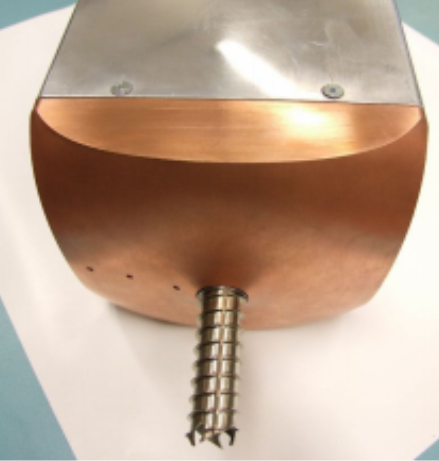
\includegraphics[width=0.45\textwidth]{figures/LAMC/iceScrew}
 	\caption{The IceMole 1 prototype using an ice screw. The copper part is the heating element and the ice screw appears in the bottom of the image. Adapted from \cite{article:dachwald2014a}}.
 	\label{fig:iceScrew}
 \end{figure}   
 
\noindent
The fourth possibility, as described by Dachwald et al (2014)\cite{article:dachwald2014a}, works by having a screw mounted on the front of the heating element. A prototype is shown in figure ,\ref{fig:iceScrew}. By rotating this screw the heater is pulled up against the ice, forcing any debris to the side. One of the big advantages of such a system is that it has a high degree of steer-ability, having even been shown to move vertically upwards\cite{article:dachwald2014a}.  
Additionally, by making the screw hollow ice cores can be made and processed inside the penetrator. Unfortunately, a number of disadvantages present themselves: The screw requires motors to rotate it, and these need to be positioned in the center of penetrator with the axle going through the heating element. This is not an issue for an electrical heater, but using RTGs would be nigh impossible in such a configuration. Furthermore, in order to provide enough torque to screw into the ice, that penetrator needs to be fixed relative to the ice. Dachwald et al achieve this by using a penetrator design with a square cross-section, however, this would not be ideal for Europa where the penetrator needs to withstand very high pressures.\\

 \begin{figure}[ht]
 	\centering
 	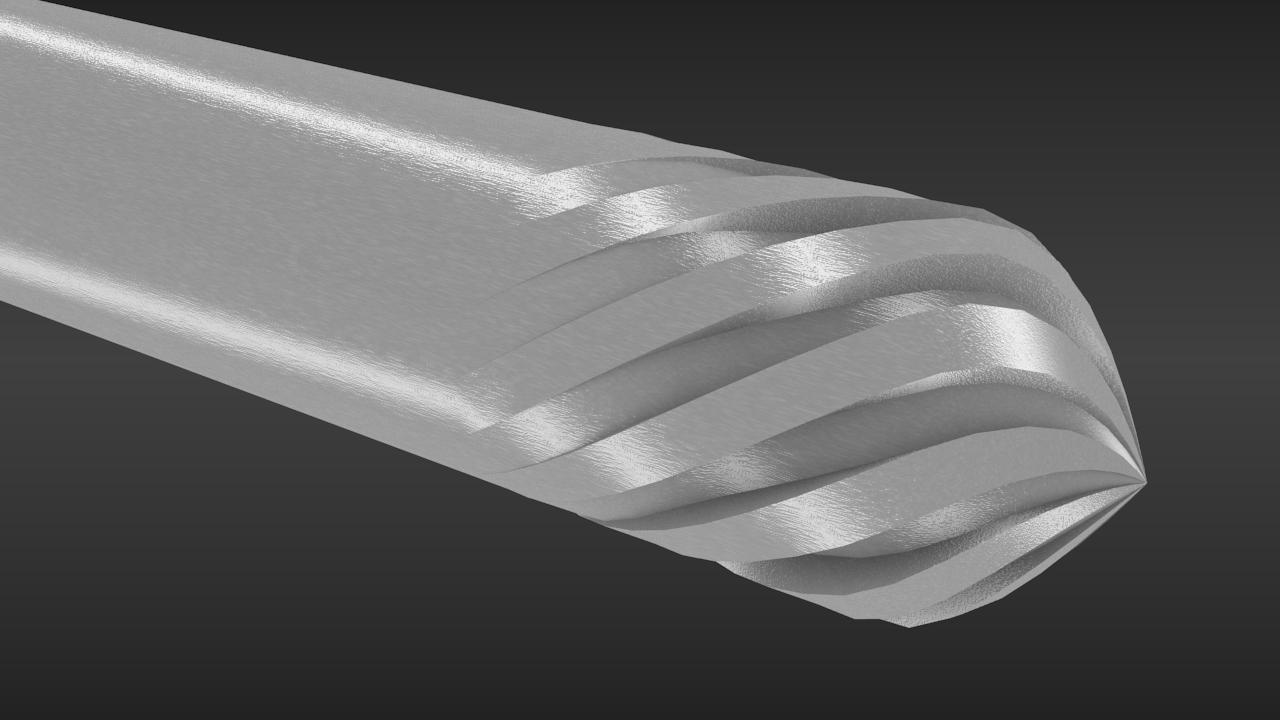
\includegraphics[width=0.5\textwidth]{figures/LAMC/flutedHead}
 	\caption{Example of how debris removal could be achieved using passive means. The flutes make the penetrator spin as it goes down, thus forcing debris to the side. This is similar to how a drill bit works.}
 	\label{fig:flutedHead}
 \end{figure}  

\noindent
The fifth method is to shape the tip of the penetrator in such a way as to remove the debris using only the motion of the penetrator itself. A way to do this is to have flutes running along the side of the device creating a shape not unlike a standard drill bit. With such a configuration, the penetrator would start to rotate as it moves downwards, and with the proper design, this will force debris to the perimeter of the bore hole following the flutes. This type of design is illustrated in figure \ref{fig:flutedHead}.  
Some issues that arise with this design include the fact that sharp edges do not work well with thermal drills, as they quickly cool down because of the large amount of heat they conduct to the surrounding. Therefore, the design in figure \ref{fig:flutedHead} would have to smoothed out somewhat, possibly reducing the debris removal efficiency. Additionally, it is hard to find examples of this design in literature, meaning that experiments are needed to determine whether it works at all. \\

\noindent
Clearly, none of these options are ideal and experiments are probably needed before a final solution can be selected. However, a combination of the third and fifth options seem like a good choice. The fluted head design cause a rotation that not only works to mitigate dust, but also works towards making the penetrator go straight down, as any unevenness that might exist in the heater will be canceled by the rotation. This combined with the water jets is likely to be able to deal with most types of debris.


\subsubsection{Future Work}

\autsection{RTG design}{Ricard Lladó Grove}

\subsection{Radiation from Pu238}
After looking at the different materials, Plutonium-238 (Pu238) is radioactive material that is going to be used for the mission due to the the half-life of 87.7 and the minimum radiation of gamma and neutrons. 

The probability of a alpha-decay from a Pu238-atom is close to 100\%: 
\begin{equation}
^{238}\text{Ph} \quad \rightarrow \quad ^{234}\text{U} \quad + \quad ^4 \text{He}
\end{equation}
The alpha particle is relatively big with two protons and two neutrons and is therefore easy to shield against. Even if the possibility of an alpha decay is close to almost certain, there is a small possibility of either a spontaneous fission or a cluster decay. A spontaneous fission happens for heavy atoms, where the atom split into two almost equal sized daughter atoms and a number of free neutrons. The possibility of a spontaneous fission for Pu238 is $1.9 \cdot 10^{-7}\%$, but with more than $10^{24}$ atoms for each kg of plutonium, it is certain to happen. The daughter atoms can vary. A cluster decay is something between an alpha decay and spontaneous decay where a cluster of protons and neutrons are emitted. For the Pu238 there is a $1.4 \cdot 10^{-14}\%$ chance that a Si32-atom is emitted leaving a Hg206-atom, and a $6 \cdot 10^{-15}\%$ chance that a Mg30-atom and a Mg28-atom is emitted leaving an Yb180-atom. The daughter isotopes are also radioactive and are most likely to emit a beta-particle. This particle is either an electron or a positron depending on the charge of the particle with a mass much smaller than neutron or proton but since it has an electric charge it can rather easily be stop by a shielding metal.\\

\noindent
A bigger problem is the free neutrons that for example are emitted due to a spontaneous fission.  The neutrons do not have any electric charge and therefore they will not be stopped by an electric field making them extremely penetrating. To stop a neutron is has to be absorbed by a nucleus or collide with a particle with same speed but opposite velocity and mass as the neutron. Since the materials used to shield alpha and beta particles, for example lead, has a rather small cross-section and hew nuclei per unit mass, hence the neutron can easily pass trough the shielding. Furthermore if the neutron is absorbed to the atom it is likely that the new atom is radioactive as well. Therefore it is important to stop the neutrons, because they can cause a lot of damage if they hit the instruments on board the penetrator. In order to do so protium, a hydrogen atom with no neutron, can be used to absorb the neutron creating in deuterium. Water has a high number density to mass ratio, and is hereby optimal to use as a shielding against the free neutrons. 


\subsection{Shielding}
As mentioned a typical shielding material is lead, but for this case zirconium would be a better choice, first of all because it has a melting temperature that is three times higher than lead, and second of all because the material is lighter. It is still not possible to stop the free neutrons, where we instead will use water. First the Plutonium will be surrounded by the zirconium, afterwards a layer of water and in the end some thermocouplers will generate electricity from the heat. 

\subsection{Heat generation}

To calculate how much energy one alpha decay will produce, the energy equation derived from Einstein is used:
\begin{equation}
\begin{aligned} 
\text{$E_{atom}$} & ={} mc^2 \\
& = (m_{Pu238} - [m_{U234} + m_{He4}]) \cdot c^2 \\
& = (238.049559894U - [234.040952088U + 4.00150646649U])\\
& \cdot 1.66053904020\cdot 10^{-27}\text{kg} \cdot 2.99\cdot 10^8 \text{m/s}\\
& = 1.06\cdot 10^{-12} J 
\end{aligned}
\end{equation}
When knowing how much one decay will produce of thermal energy, the number of decays in a radioactive material can be calculated as following:
\begin{equation}
A = A_0 \cdot 2^{\frac{t}{\tau}}
\end{equation}
where \textit{$A_0$} is the initial number of atoms in a lump of a radioactive material, \textit{A} is the atoms left in the material after a specific time, \textit{t}, with a half-life of  \textit{$\tau$}. The energy produced by one kg of Pu238 over a timespan of one second will then be: 
\begin{equation}
\begin{aligned} 
\text{$E_{kg}$} & ={} E_{atom} \cdot [A_0 - A] \\
& = E_{atom} \cdot \left[A_0 - A_0 \cdot 2^{\frac{t}{\tau}}\right] \\
& = E_{atom}  \cdot \left[\frac{1}{m_{Pu238}} - \frac{2^{\frac{t}{\tau}}}{m_{Pu238}} \right] \\
& = 671 J
\end{aligned}
\end{equation}
We here see that for each kg of Pu238, 671W energy is generated in form of thermal energy. Since the amount of Pu238 decreases for each decay, the generated energy will also decrease, but rather slowly since the half life is 87.7 years. 
After the decay to U234, the uranium is also radioactive, undergoing an alpha decay as well. The lifetime is more than 2400 years and therefore the decay from this isotope is much more protracted. The decay chain from Pu238 will end with the stable isotope Pb206 after 12 decays from either alpha or beta decay. \\

\noindent
Since we need 2kW of thermal energy and around 100W as electrical energy for the instruments on the penetrator we would need around 5 kg of plutonium. Some extra plutonium is needed because the amount of radioactive material decreases with time, and since the mission takes a couple of years the heat generation have decreased a factor 
\begin{equation}
N = N_t \left(\frac{1}{2}\right)^{t/\tau} 
\end{equation}

\noindent
With a density of 19816 kg$/m^3$, with a mass of 5 kg we would need a a plutonium rod that is 30 cm long and 1.65 cm in radius. It is a good idea that the plutonium has a high surface area compared to the volume, because the heat was to be distributed to the water running in the heat pipes(maybe). Furthermore it is a good thing that the plutonium has the same shape as the penetrator. (Explanation to come) 


\subsection{Heat pipes}
To distribute the heat that is generated from the plutonium. In order to do so, the water will be under high pressure. If the pressure inside the pipe system is 50 bar, or around 5 MPa, the water has a boiling temperature at $264^\circ$C. This will give some advantages for the system in the sense that it is almost impossible to maintain a temperature below $100^\circ$C which is waters normal boiling point, when transporting 2kW of heat.\\

\noindent
The pipe system will consist of pipes surrounding the RTG in the bottom and middle of the penetrator. Since the RTG is 30 cm long the pipes will be this as well with 18 tubes cut in half. The water will then flow out to the 18 tubes in the outer part of the RTG. Since most of the heat of generated should be directed downwards 12 of the tubes only cover the lowest $1/4$ of the penetrator. The other 6 tubes will go all the way to the top of the penetrator in order to ensure that the penetrator will not freeze in because the top of the penetrator is too cold. With an internal pressure of 5MPa, the thickness of the tubes that have water in them will be around 1 mm depending on the material if the other radius of the tubes are 1.48 cm. The heat pipe system will then weight around 6 kg. Furthermore the system will take up 6.5 liters of space. 

Insert image of top view of the pipe system and RTG. 
Insert image of a sideways look of the system.

\autsection{Pressure Distribution Europa}{Ricard Lladó Grove} 

Secondly the gravitational acceleration is set to be $1.314 \frac{m}{s^2}$, and has been calculated by 
\begin{equation}
g = \frac{GM}{r^2}
\end{equation} 
where $G = 6.67\cdot 10^{-11}\frac{m^3}{s^2 kg}$ is the gravitational constant, $M = 4.8\cdot 10^{22}$kg is the mass of Europa and $r = 1560.8$ km is the radius of Europa.  We see that the further the penetrator melts its way down through the ice the radius decreases. The mass distribution will also change since now there will be mass above you which will pull you in that direction, but on the other hand you will be closer to the mass on the other side of the planet. Therefore the change in gravitational acceleration depends on the distribution of the mass on Europa, and especially how dense the core is which in this case is unknown. 



\section{Selected Design}

* Sketch of overall design (use 3D models for the ice melting simulations)

\subsection{Melting through the ice} % Lukas, KSL

\subsection{RTG on Top}

\subsection{RTG on Bottom}

* How do we protect the rest of the instruments against the radiation?


\subsection{Thermal Design}

\subsection{Water Convection}

\section{Anchor Design}
\autsubsection{Buoyancy}{Ricard Lladó Grove}
One way to anchor the penetrator is through buoyancy. In general buoyancy is an upward force that is exerted to an object by the surrounded fluid. For an object immersed in a fluid, the force acting on the object is gravity and buoyancy given by:
\begin{subequations}
\begin{equation}\label{eq:bouyancy1}
F_{gravity} = m_{object} \cdot g
\end{equation}
\begin{equation} \label{eq:bouyancy2}
F_{buoyancy} = \rho_{fluid}\cdot g \cdot V_{immersed} 
\end{equation}
\end{subequations}
where $g$ is the gravitational acceleration, $\rho$ is density, $V$ is volume of the immersed part of the object and $m$ is mass.  In our case the object is the penetrator and the fluid that the penetrator is immersed into is assumed to be pure water. In order to use buoyancy as the anchor of the penetrator, it has to cancel out the force of the gravity that will pull the penetrator downwards i.e make it sink. We can hereby equal equation \ref{eq:bouyancy1} and \ref{eq:bouyancy2}:
\begin{subequations}
\begin{equation*}\label{eq:bou1}
F_{gravity} = F_{buoyancy} \quad \rightarrow \quad m_{penetrator}\cdot g_{Europa} = \rho_{fluid}\cdot g_{Europa} \cdot V_{immersed}   \quad \rightarrow 
\end{equation*}
\begin{equation} \label{eq:bou2}
V_{immersed} = \frac{m_{penetrator}}{\rho_{fluid}}
\end{equation}
\end{subequations}
First of all we see that the gravitational acceleration of Europa cancels out in both equations, which simplifies the expression. It is desired to calculate the volume that is needed in order to the force of the buoyancy to be great enough to lift the mass of the penetrator hence cancel out the gravity. The mass of the penetrator is in our mission straw man set to be maximum 180 kg even though it is only an assumption  If the mass of the penetrator shows to actually be lower than expected a lower volume would be needed. The density of the water is set to 1000 $\frac{m^3}{kg}$ which is the density of pure water. It is not known how salty the water if it contains salt, but the density of salt water is slightly higher then water without salt, and hereby the buoyancy force would be higher and a smaller volume is needed, so by using pure water we get a conservative value of the volume. By inserting the value we end up with the volume needed to carry the penetrator in pure water:
\begin{equation}
V_{needed} = 0.180 m^3 \rightarrow 180 \text{litres}
\end{equation}
Since the penetrator is 48.2 litres the extra required volume is about 132 litres. When the penetrator melts through the last ice the velocity of the penetrator will increase because the it will sink though the water. With a short delay to ensure that the penetrator is surrounded by water, a trigger should inflate a balloon attached to the penetrator. The balloon should have a volume of at least 132 litres since we would probably like a small lift of the buoyancy. 
\begin{figure}[htb]
  \centering
  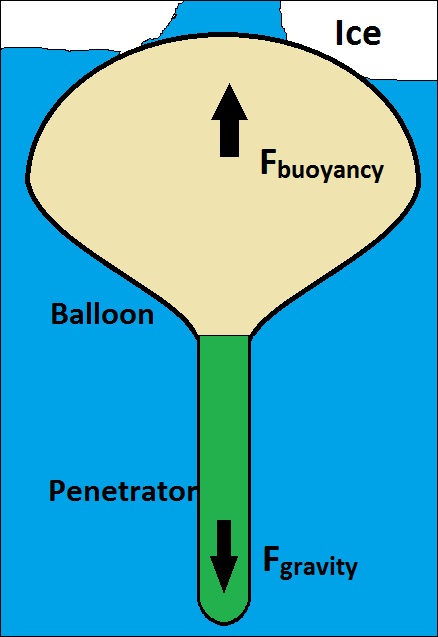
\includegraphics[width=0.5\textwidth]{figures/Ricardo/Buoyancy1.png}
  \caption{Illustration of the immersed penetrator with the inflated balloon to reach equilibrium between the buoyancy force and the gravitational force}
  \label{fig:buoyancy1}
\end{figure}
\noindent 
The next thing is to find out what gas could be used in the balloon and how much of it is needed. Here one big problem of the buoyancy solution to anchor the penetrator arises, namely that almost all gases are liquid or solid at really high pressures. If for instance using CO2 as the gas used inside the balloon the phase diagram can be seen in figure \ref{fig:CO2phase}.
\begin{figure}[htb]
  \centering
  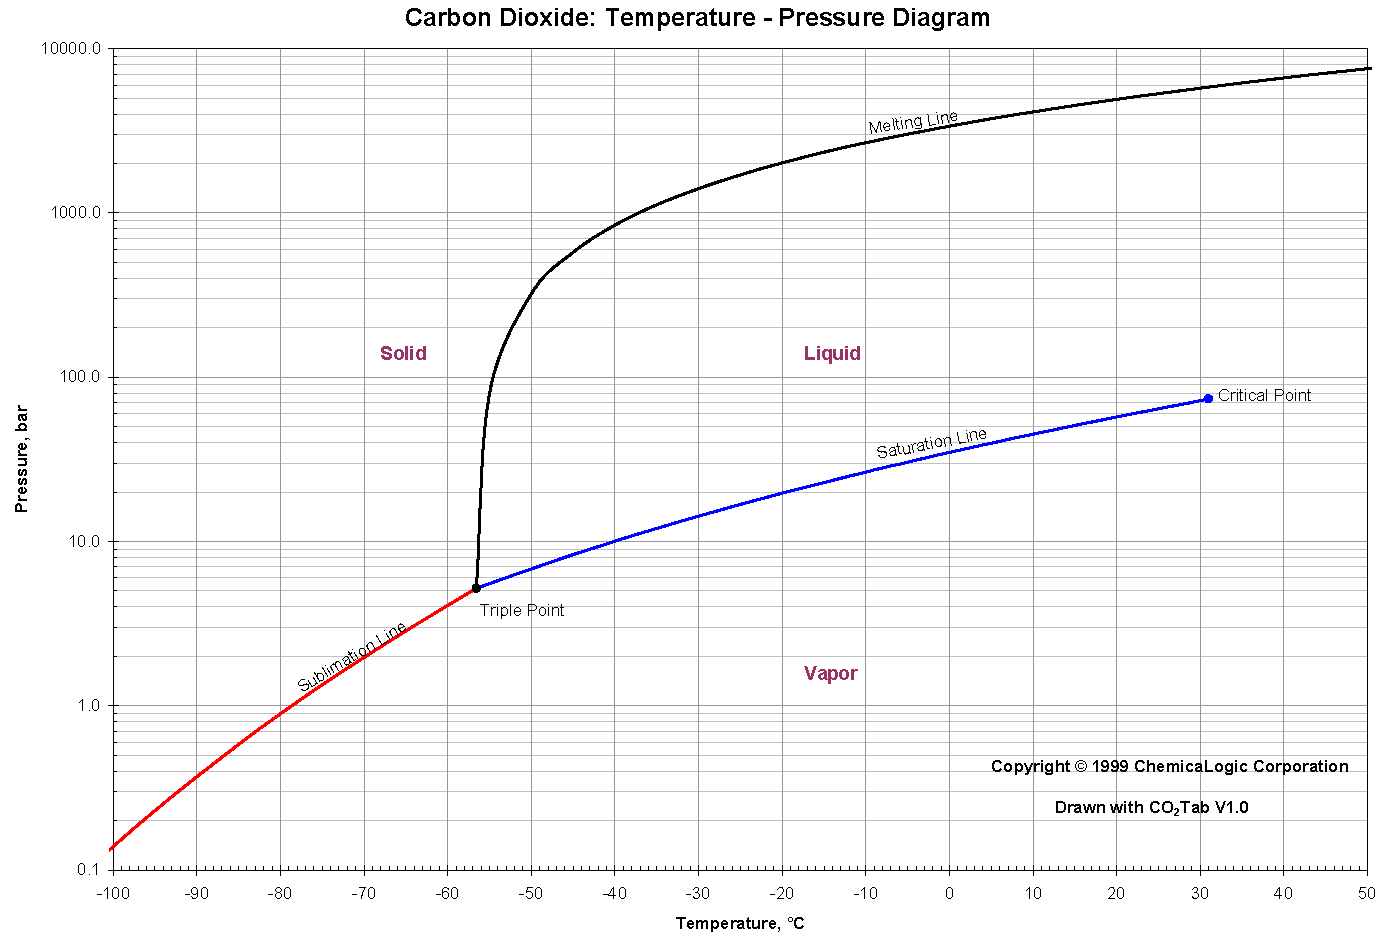
\includegraphics[width=0.9\textwidth]{figures/Ricardo/co2_phase_diagram}
  \caption{Phase diagram of CO2. From: \url{http://www.chemicalogic.com/Documents/co2_phase_diagram.pdf}}
  \label{fig:CO2phase}
\end{figure}
If assuming that the balloon will be above the penetrator which is the preferred way since the density of the gas will be less compared to the one of the penetrator. Hereby we will have a more stable structure. Hereby the temperature of the gas would be almost the same as the temperature of the surrounding water which is around 273 K, corresponding to $0^oC$. In figure \ref{fig:CO2phase} the vaporization point corresponding to this temperature is 35 bar. Since we have to assume the worst case scenario the depth of the ice could be up to 10 km deep, and as calculated in an earlier section the pressure will at this depth be 12MPa which is approximately 120 bar. Therefore the CO2 will vaporize and the volume decrease. In order to have CO2 on gas form at this high pressure a higher temperature of the gas is needed. The critical point for CO2 is about $30^oC$ where the pressure is just above 70 bar. This means that another gas has to be used in order to make buoyancy work at this pressure. For water the phase diagram is illustrated ealier we see that at temperatures around 600 Kelvin the vaporization point is about 120 bar. A possible solution these high temperatures would be to have the balloon surrounding the penetrator and use the heat produced by the RTG to warm up the gas. This would produce problems since the density of the gas would be less than the density of the penetrator and hereby in worst case scenario the penetrator would flip up side down and all communication would be lost. Furthermore the heating of the gas would last for relatively long time and hereby the penetrator would have sunken before the force of the buoyancy would be great enough to lift the penetrator. Therefore the solution with a heated gas would not work. Now assuming that the ice layer is only two kilometres deep the pressure would be around 34 bar which is just below the vaporization point for CO2 at $0^oC$. To get an estimate of how much CO2 is needed if assuming that the penetrator should be anchored at 2 km depth, the the ideal gas law can be used, which is given by equation \ref{eq:idealgaslaw}. 
\begin{equation} \label{eq:idealgaslaw}
PV = nRT
\end{equation}
where $P$ is pressure, $V$ is volume, $n$ is how many moles is in the gas, $R$ is the ideal gas constant and T is temperature. Since CO2 weights 44 gram per mole it is possible to calculate the mass for 132 litres of CO2: 
\begin{equation}\label{eq:massCO2}
m_{CO2} = \frac{M_{CO2} \cdot P_{water}\cdot V_{balloon}}{R\cdot T_{water}} = \frac{44 \frac{g}{mole} \cdot 35 bar \cdot 132 L}{0.0831  \frac{L\cdot bar}{mole \cdot K} \cdot 273K} = 882.8 g
\end{equation}
From equation \ref{eq:massCO2} it is seen that only 0.882 kg CO2 is needed with a pressure of 35 bar, but if the pressure would increase to 120 more CO2 is needed in order to withstand the higher pressure. One way to produce CO2 is to burn octane: 
\begin{equation}
2 C_8H_{18} + 25 O_2 \rightarrow 18 H_2O + 16 CO_2
\end{equation}
It can be seen that in order to get 0.88 kg of CO2 through burning of oxygen more mass is needed than the CO2 produced. A rough estimate of the the total octane and oxygen is about 1.5 kg  which is also included in the 180 kg of the maximum weight of the penetrator. What has not been taken into account is the material that the balloon is made of. It has to be a really strong material since there the balloon will be in contact with the ice. Depending on how point the ice will be, it can make a hole in the balloon which will be critical since the mission will fail if this happens since the penetrator will sink, and since it is not made to be able to withstand higher pressure than at 10 km depth it would start to buckle and furthermore the communication will also be lost. Besides being really strong the material has to be flexible because it should not take up all the penetrators space when not inflated, but be able to expand. This will not be discussed further either since buoyancy is not the chosen anchoring method. Another problem is that in order not to lose communication with the lander the communication system should be on top of the balloon if the balloon is above the penetrator, which is doable but really unhandy. If the communication should not be lost it is also desired that the penetrator does not drift because of the current in the water in Europa, so a system should also be designed to grip the ice and fix the position of the penetrator.\\

\noindent
One of the biggest problems is that at 10 km depth which is the maximum depth that is expected the pressure is too high for a molecule to be in gas form and would instead be in liquid or a supercritical fluid where no phases exist. Therefore the buoyancy does not work at such depth but they have a potential for a depth of around 2 km. For this mission it is important not to have a mission killer and therefore buoyancy is a bad solution for anchoring the penetrator which is also the reason why no more designing has been made of the the ignition of CO2, time of filling up the balloon, material decision and antenna design so we do not lose communication with the lander. 

\autsubsection{Polypropylene foam}{Paul Connetable}

\subsubsection{Capabilities of polypropylene foam}

Another possibility for anchoring the penetrator to the ice layer is to use polypropylene foam. Polypropylene foam is a hardening foam, it can be stored at a high pressure and low temperature for a long time. When needed, it is possible to make it expand by increasing its temperature and releasing it into a wider, open space. The expansion of the foam is made thanks to the expansion of a gas contained in the polymer melt. This gas, called blowing agent, creates bubbles in the polymer, which expand and make the foam expand. During the process, the density of the foam lowers, and it crystallizes, becoming harder and rigid.

The concept idea of using a hardening foam to anchor the penetrator to the ice is that the foam can be stored in a ring around the penetrator, like a buoy. When the penetrator needs to be anchored, the foam could be heated up thanks to the heat produced by the RTG, and released in the penetrator's surroundings, by opening apertures in the ring. This way, the foam would expand and crystallize both inside and outside the buoy of the penetrator. The foam could then expand in the hole drilled, and get in contact with the ice matrix. If the ice has asperities or holes, or is slushy, the foam could then follow the ice profile, and offer a resistance to the penetrator descent, by clinging on to the ice.

The polypropylene foams seem to be well suited for our very specific use and the extreme conditions found at the bottom of Europa's ice crust. Moreover, some research has been done in \cite{naguib2002strategies}, to improve drastically some parameters of polypropylene foams. Some of the results found on this study are presented here. In particular, in this paper, the expansion ratio, the foam density in Figure, and the blowing agent pressure are presented for several chemical compositions of the foam in function of the melt temperature. These results are respectively shown here in Figures \ref{foamexpansion}, \ref{foamdensity} and \ref{foampressure}.

\begin{figure}[H]
\begin{center}
%\fbox{
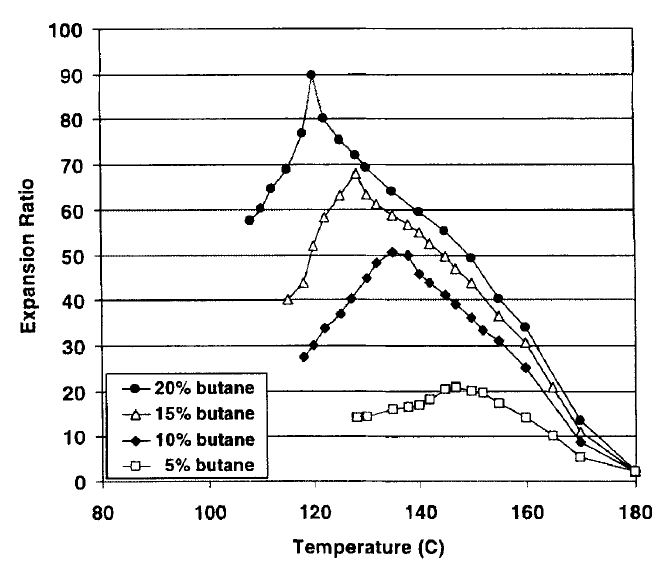
\includegraphics[width=10cm, height=8cm, clip]{figures/Paul/foamexpansion.JPG}
%}
\end{center}
\caption{Expansion coefficients of branched polypropylene material, for different temperatures and material compositions}
\label{foamexpansion}
\end{figure}

\begin{figure}[H]
\begin{center}
%\fbox{
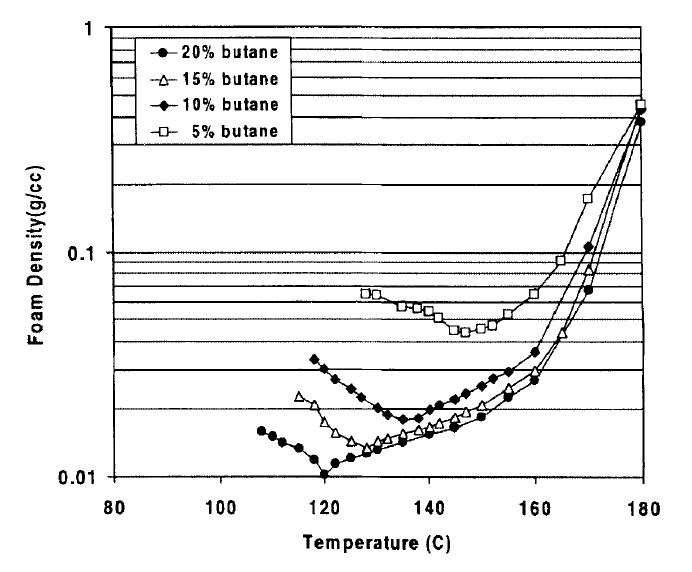
\includegraphics[width=10cm, height=8cm, clip]{figures/Paul/foamdensity.JPG}
%}
\end{center}
\caption{Foam density of branched polypropylene material, for different temperatures and material compositions}
\label{foamdensity}
\end{figure}

\begin{figure}[H]
\begin{center}
%\fbox{
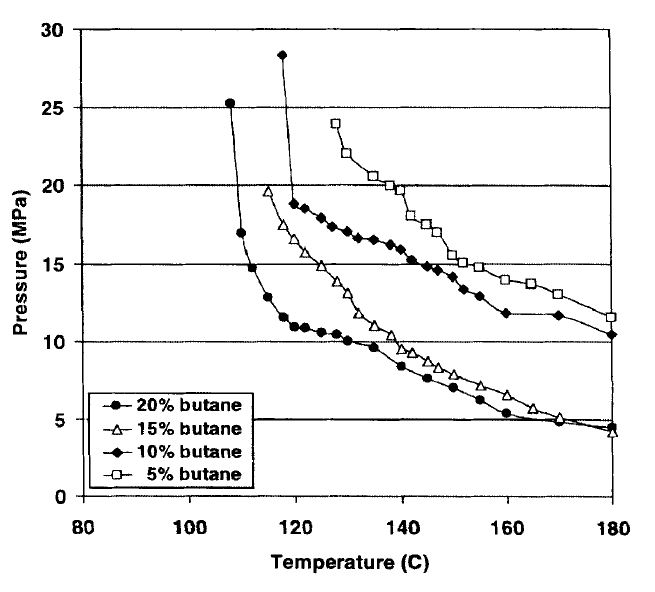
\includegraphics[width=10cm, height=8cm, clip]{figures/Paul/foampressure.JPG}
%}
\end{center}
\caption{Blowing agent die pressure, for different temperatures and material compositions}
\label{foampressure}
\end{figure}


The first interesting result is that, as presented in Figure \ref{foampressure}, the working pressure of the blowing agent in the foam is very high. Even though this working pressure goes down if the butane percentage increases, it is greater than the pressure at 10~km depth under the ice crust on Europa, which is of only about 12~MPa. It means that this kind of foam has a working pressure high enough to still expand in this situation, if the foam temperature is not too high.
Secondly, one can see in Figure \ref{foamdensity} that the foam density is quite low. It is possible to cross this information with Figure \ref{foamexpansion} to find out that the density of the stored product is of about 1 $kg/dm^{3}$, as water. it means that bringing foam would be moderately heavy. However, for reasons explained below, assessing precisely the quantity of foam needed is impossible right now. Finally, as it can be seen in Figure \ref{foamexpansion}, the expansion of the material tested on Earth at 1 bar is very impressive and promising.

\subsubsection{Conclusion on this method}

Anchoring the penetrator thanks to polypropylene foam seems interesting, thanks to some good points of this method. It has indeed the possibility to work at 12~MPa pressure and at the 0°C temperature, thanks to the heat emitted by the RTG. Moreover, since the heat could be obtained thanks to the RTG, it is possible to monitor precisely the temperature of the foam, which is the main variable in its expansion. Since the foam is impermeable, it can be used in water without any problem. It also gives the possibility to anchor in slushy ice, which is not the case of some other methods.


However, it still has some flaws. The most important one is that this anchor could only be used once. This means that it could not be possible to detach the penetrator from its position if the anchoring was not done at the right place, for example if it anchored on the top of lake in the ice crust and not on the ocean. The anchoring would also not be instantaneous but take up to several dozens of seconds to work.
Moreover, no study has been done about anchoring with expanding foam. Therefore, there is today no way to ensure the reliability of this method, or to quantify the amount of foam needed to attach the penetrator to the ice, or the variation of this quantity with the characeristics of the ice, such as its chemical composition, its temperature, its slushiness. There is even the possibility that the heated foam could make the ice melt at its contact and therefore, not being able to anchor the penetrator properly.

This shows that anchoring the penetrator thanks to expanding foam is a very serious lead, as it is very promising, and could be able to anchor the penetrator to slushy ice. However, since absolutely no research has been done on this subject, any quantification or even proof of concept is today impossible to bring.




\subsection{Anchoring and Deployment}

* Ref to composition of the ice and theory about lakes?

\section{Mechanisms and Instrumentation}

\subsection{Navigation and Dirigeability}

\subsection{Submarine}

\subsection{Detection of Depth and End of Ice Column}

* Echo sounder etc

%\section{Communication Systems}

%\subsection{Communication to Lander}

%\subsection{Relay Systems}
